\chapter{Introduction}

Wide-area streaming analytics are becoming pervasive, especially with the
emerging Internet-of-Thing (IoT) applications. Large cities such as New York,
Beijing and Seattle are deploying millions of cameras for traffic
control~\cite{london.surveillance,skynet}. Retails stores and critical areas
such as railway stations are also being monitored for abnormal
activities. Buildings are increasingly instrumented with a wide variety of
sensors to improve building energy use, occupant comfort, reliability and
maintenance~\cite{krioukov2012building}. Geo-distributed infrastructure, such as
Content Delivery Network (CDN), needs to analyze user requests (machine logs)
and optimize data placement to improve delivery efficiency. In these problems,
the data collected at the edge needs to be transported acoross the wide-area and
analyzed in real-time.

Existing stream processing for ``big data,'' such as
Storm~\cite{toshniwal2014storm} or Spark
Streaming~\cite{zaharia2012discretized}, only work in the context of a single
cluster, where the bandwidth is sufficient (or at least easy to
provision). While they are the perfect back end for analyzing streams once data
arrive, in the wide-area, the network, with scarce and variable bandwidth,
easily becomes the bottleneck \cite{rabkin2014aggregation}. What's worse, the
growth rate of wide-area network capacity is not keeping up with the increasing
rate of traffic~\cite{index2013zettabyte}.

When facing situations where the bandwidth is not sufficient, applications
deployed today either choose a conservative setting (e.g.\,only delivering 360p
videos) or leave their fate to the underlying transport layer: (1) in the case
of TCP, the sender will be blocked and data are backlogged, leading to severe
delay; (2) in the case of UDP, uncontrolled packet loss occurs, leading to
application performance drop. Instead of ``suffering'' from a degraded network,
applications can act proactively by adjusting their behavior: reducing the data
rate to ensure that important data are delivered in time.

The idea of adapting data rate for data freshness is not new. Multimedia
applications and their adaptations~\cite{michalos2012dynamic,
  schulzrinne1998real} have been extensively studied in the past because their
high demands on the network are rarely met. However, since their goal is to
improve \textbf{user experience}, their adaptation strategies are not
necessarily optimal for streaming analytics. For example, humans can tolerate
loss on video frame details but expect a smooth frame transition---at least 25
frames per second (FPS). But many vision analytics are based on algorithms that
extract edge information from a frame---they will perform poorly if frame
details are lost after an aggressive quantization.

The observation that different applications demand different strategies in order
to achieve the optimal adaptation calls for a system-level approach. In this
proposal, I present the design and implementation of \sysname{}, an adaptive
stream processing system for the wide-area. Under normal operations, \sysname{}
applications work with maximal data fidelity; when the network's capacity
changes, applications will react by controlling the level of
\textbf{degradation}: trading data fidelity for freshness.

Although the basic idea behind degradation is intuitive, realizing them in
practice is non-trivial. Firstly, as has been discussed earlier, different
degradations have different impacts across applications and data
distributions. Secondly, each degradation is often more than a binary decision;
they can be parameterized with a wide range of tuning space. It's not always
possible to derive a close-form analytical relationship between the degradation
parameter and its impact on the bandwidth and accuracy. What's more, real-world
applications often have multiple dimensions to tune---prohibiting a manual
exploration of all the design space. Take video analytics as an example,
reducing image resolution, frame rate or changing the video encoding quality are
all possible degradation operations. Each operation will affect data rate and
application accuracy but its impact to the video quality is not immediately
obvious for developers. The situation is worse when multiple degradations are
employed. These challenges are elaborated in~\autoref{sec:challenges}.

To address the challenges, \sysname{} employs a data-driven empirical-analysis
approach that's analogous to machine learning.  First, \sysname{} separates
application logic from adaptation strategies by providing a clean abstraction
(\texttt{maybe} APIs) for developers: this allows expressibility without
burdening the developers for an exact strategy. \sysname{} then profiles the
application using representative datasets and application-specific utility
functions to ``learn'' the optimal strategies under different network
conditions. The profile is then used to guide the runtime adaptation, for which
\sysname{} provides all the necessary ``plumbing'' modules to without
application developers' effort. In \autoref{sec:architecture}, I will present a
detailed description of \sysname{}'s architecture.

To study and validate the effect of degradation, I've built a prototype
framework and three real-world applications using \sysname{}: a street
surveillance application performing pedestrian detection, an augmented reality
application recognizing everyday objects and a distributed top-k application
analyzing web server access logs. The first two video streaming applications
have three degradation operations: reducing resolution, frame rate and video
encoding quality. For the distributed top-k application, two degradation
operations are envolved: N in a local top-N operation and T as a local
threshold. \autoref{sec:build-appl} discusses the considerations and details
about the prototype.

The evaluation shows that the offline profiling is able to explore the design
space for all three applications and generate the Pareto-optimal adaptation
strategies that was not achievable with manual developer configurations or with
only a single degradation operation. These profiles offer a quantitative
understanding of each application's behavior. During runtime, \sysname{}
applications are compared against traditional transport protocols including TCP
and UDP with a controlled experiment. When the network capacity drops, TCP
creates a severe delay; and the delay increases linearly as time goes; for UDP,
a severe packet loss makes the application unusable. Applications built with
\sysname{} handles the network variation gracefully: video streaming analytics
is able to keep the latency bounded with 2 seconds and the accuracy higher than
80\%. For the top-k application, although the feedback is less frequent and
adaptation is not always immediate, the worst-case latency is 12 seconds at most
and the accuracy is mostly above 75\%.

To this end, this thesis makes the following contributions:

\begin{itemize}
\item An in-depth study of wide-area streaming applications in the case of
  network resource variation.
\item The proposal of novel APIs to allow for a design space exploration between
  bandwidth and accuracy with minimal developer effort.
\item A prototype implementation that demonstrates application profiling and
  runtime adaptation.
\item Thorough evaluations based on three real-world applications under
  different scenarios.
\end{itemize}

\section{Motivating Applications}
\label{sec:motiv-appl}

There is a variety of wide-area streaing applications. We discuss three
applications with their implications.

\para{Video Surveillance:} We envisage a city-wide monitoring system that
aggregates camera feeds (both stationary ground cameras and moving aerial
vehicles) and analyzes video streams in real-time for surveillance, anomaly
detection or business intelligence~\cite{oh2011large}. While traditionally human
labors are involved in analyzing abnormal activities, recent advances in
computer vision and deep learning has dramatically increased the accuracy for
automatic analysis of visual scenes, such as pedestrian
detection~\cite{dollar2012pedestrian}, vehicle tracking~\cite{coifman1998real},
or facial recognition to locate people of
interest~\cite{Lu:2015:SHF:2888116.2888245, parkhi2015deep}.
% \cite{gantz2012digital}

\para{Electrical Grid Monitoring:} While traditional environmental sensors are
slow~\cite{atzori2010internet}, we are seeing an increasing trend with
high-frequency, high-precision sensors being deployed. For example, the
microsynchophasors monitoring system for the electrical grid consists of a
network of 1000 devices; each produces 12 streams of 120 Hz high-precision
values accurate to 100 ns. This amounts to 1.4 million points per second that
requires specialized timeseries database~\cite{andersen2016btrdb}.

\para{Log Analysis:} Large organizations today are managing 10--100s of
datacenters (DCs) and edge clusters worldwide~\cite{calder2013mapping}. While
most log analysis today runs in a batch mode and at most on a daily basis, there
is a trend in analyzing logs in real time for quicker
optimization~\cite{alspaugh2014analyzing}. For example, by analyzing the access
logs in real time, a content distribution network (CDN) can improve the overall
delivery efficiency with optimized data placement.

\vspace{0.5em}

These applications share a similar structure: a large volume of data generated
at the edge need to be transported across the wide area network for real time
analysis. Because of the limited network resources in the wide area, they will
face practical issues when deployed at a scale.

\section{Wide-Area Bandwidth Characteristics}
\label{sec:making-case-adapt}

\begin{figure}
  \centering
  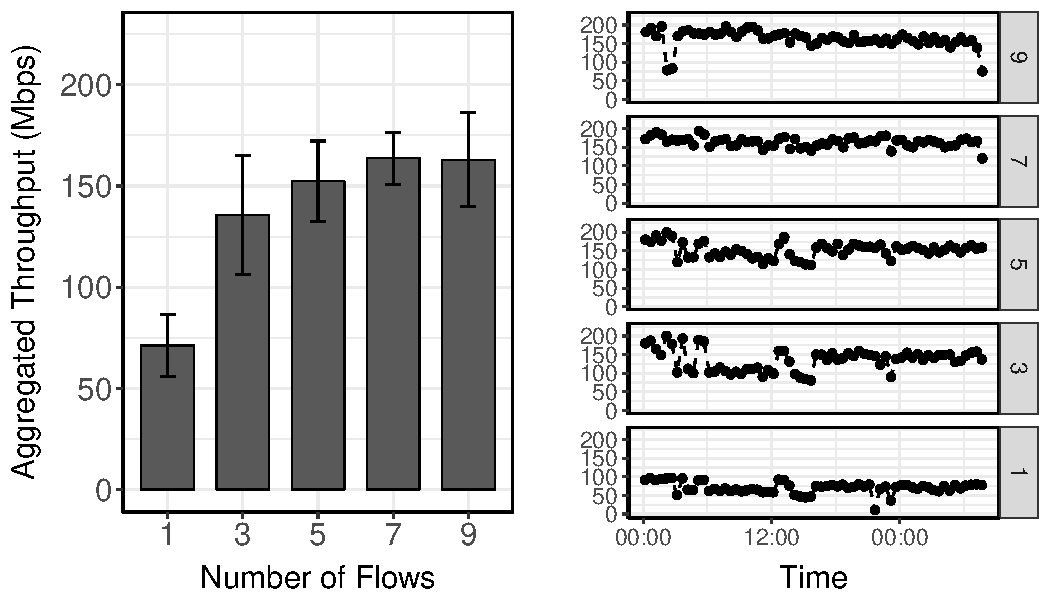
\includegraphics[width=.95\linewidth]{figures/europe-to-us-west.pdf}
  \caption{Bandwidth measurement between Amazon EC2 sites (from Ireland to
    California). Note the time-series plot has a resolution of 30 minutes; each
    point is more than a short period of transient degradation.}
  \label{fig:bw}
\end{figure}

To understand the bandwidth characteristics in the wide-area, I conducted a
simple measurement using Amazon EC2. iPerf~\cite{iperf} was used to measure the
pair-wise bandwidth between four geo-distributed sites throughout the day. The
measurement shows large variance in the measured bandwidth and one such pair of
sites is shown in \autoref{fig:bw}. Regardless of the number of
flows\footnote{EC2 has a per-flow and per-VM rate
  limiting~\cite{zhang2016guaranteeing}.}, there exist occasions when the
available bandwidth is almost halved. Generally speaking, the back-haul links
between EC2 sites are better (if not at least representative) in comparison to
the overall wide-area link quality. This varying nature poses real challenges to
the realization and successful deployment of wide-area streaming applications.

\section{Making the Case for a System Approach}
\label{sec:bat}

When facing insufficient network bandwidth, applications that do not adapt will
suffer severe performance penalty: such as a backlog of data for TCP or
uncontrolled packet loss for UDP. Instead of giving up control to the underlying
transport layer, applications can react and adapt their behaivors to the
resource changes.

While adaptive streaming exists in certain application domains, there has not
been a general solution. Consider video streaming applications that have been
extensively studied in the literature. There are a plethora of encoding
techniques~\cite{richardson2011h, grange2016vp9} with adaptive
strategies~\cite{yin2015control, michalos2012dynamic, pantos2016http}, however,
their primary goal is to optimize end-user quality of experience (QoE).  When
end users consume a video clip, a smooth video is often more enjoyable than
videos with intermittent pauses, even though each pause has crisp images.

Optimizing for QoE doesn't work for our target applications. Each video
analytics has its own goal, entailing different adaptive strategies for
different applications. For example, some computer vision detection algorithms
rely on the edge information~\cite{canny1986computational, lowe2004distinctive,
  viola2001rapid} while object tracking applications works best when the
inter-frame difference is small~\cite{allen2004object}.

\begin{figure}
  \centering
  \includegraphics[width=\linewidth]{figures/image-example.pdf}
  \caption{The frame difference between two images with one second difference.
    These are two different deployment scenarios: a stationary camera in a far
    field (upper) and a mobile camera for nearby objects (lower). The solid
    rectangle in each scene is the detection target; the dotted rectangle on the
    right side mirrors the detection on the left side. }
  \label{fig:image-eg}
\end{figure}

Furthermore, even similar applications, when used in different context, require
different strategies. \autoref{fig:image-eg} offers an example. The pedestrian
detection is deployed on a ground stationary camera in a far-field view. When
taking pedestrian walking speed into consideration, there is so little
difference between frames that it's not necessary to guarantee a high frame
rate. But because the camera is far from the targets, it's crucial to have a
high-resolution and sharp image. On the other hand, object recognition on a
mobile phone captures nearby objects. Due to the movement of the camera,
reducing frame rate will introduce significant errors. \autoref{fig:motiv} shows
the different rate in accuracy drop when image resolution or frame rate is
reduced for the two use cases.

\begin{figure}
  \centering
  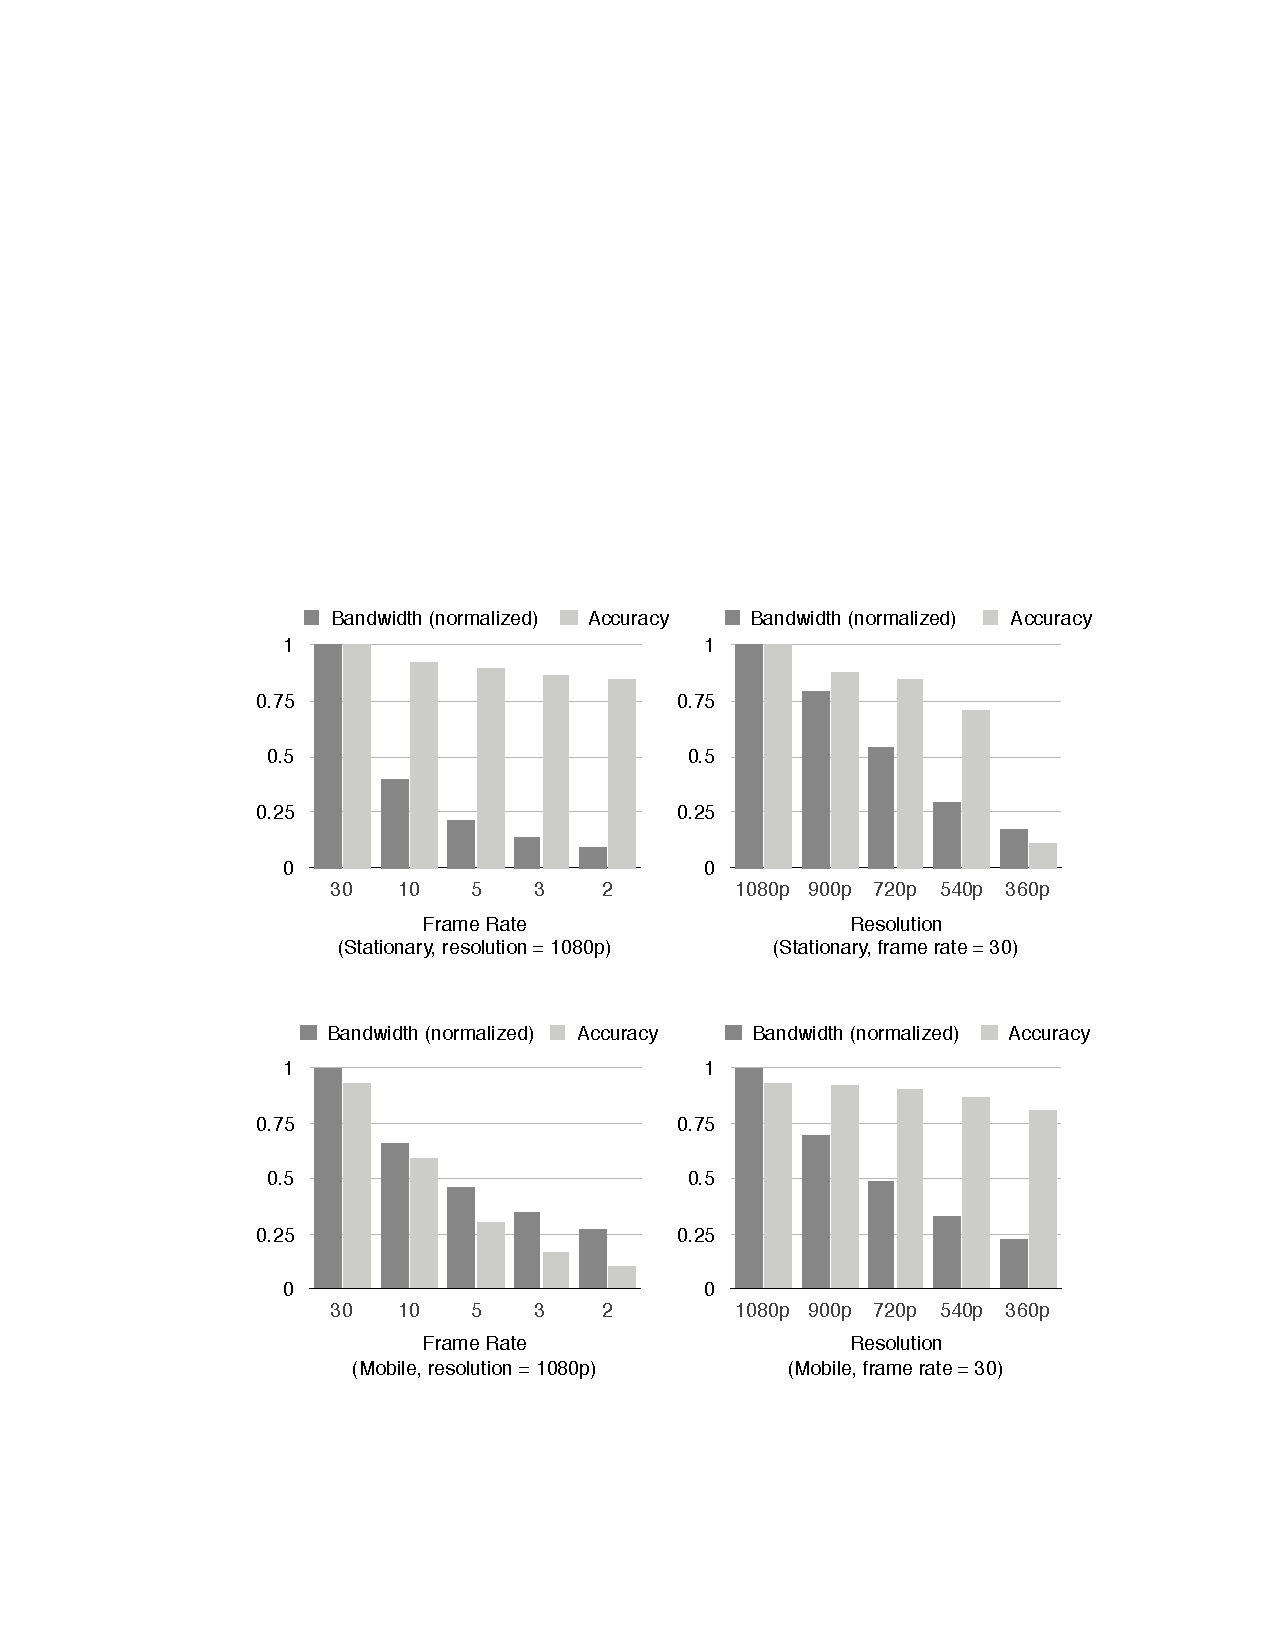
\includegraphics[width=\linewidth]{figures/motiv.pdf}
  \caption{Horizontally, how reducing the frame rate or resolution affects the
    bandwidth requirement and appliation accuracy. Vertically, how the same
    degradation have different impact for different data characteristics; the
    upper figures are for a stationary camera deployment while the lower figures
    are for mobile applications.}
  \label{fig:motiv}
\end{figure}

This motivates us to take a system-level approach that synthesizes different
adaptation strategies for different queries and contexts.

\section{Related Work}
\label{sec:related-work}

\paraf{Stream processing systems:} Streaming databases, such as
Borealis~\cite{abadi2005design},
TelegraphCQ~\cite{chandrasekaran2003telegraphcq}, are the early academic
explorations. They pioneered the usage of dataflow models with specialized
operators for stream processing. Recent research projects and open-source
systems, such as MillWheel~\cite{akidau2013millwheel},
Storm~\cite{toshniwal2014storm}, Heron~\cite{kulkarni2015twitter}, Spark
Streaming~\cite{zaharia2012discretized}, Apache Flink~\cite{carbone2015apache},
primary focus on fault-tolerant streaming in the context of a single
cluster. While this thesis has a large debt to the prior streaming work,
\sysname{} is designed for the wide-area and explicitly trades data fidelity for
data freshness; many other stream processing systems choose to throttle the
source when backpressure happens~\cite{kulkarni2015twitter}.

\para{WAN-aware:} There is a growing interest in building systems that optimizes
data transfers for the wide area, such as GDA~\cite{pu2015low},
Clarinet~\cite{viswanathan2016clarinet} and OWAN~\cite{jin2016optimizing}.  Most
of these works focus on one-time queries or operations (such as data
transfer). JetStream~\cite{rabkin2014aggregation} is the first that studies
streaming analytics in wide area and proposes to use structured storage (data
cubes) and explicit degradation policies. While JetStream has demonstrated
application responsiveness with hand-written degradation policy, these policies
are often developer heuristics that are not backed up by measurements. This
thesis extends the idea of degradation with an automatic policy synthesis.

\para{Approximate analytics:} The idea of degrading computation fidelity for
responsiveness has also been explored in other contexts, primarily SQL
queries. Online aggregation~\cite{hellerstein1997online},
BlinkDB~\cite{agarwal2013blinkdb} and GRASS~\cite{ananthanarayanan2014grass}
speed up queries with partial data based on a statistical model of SQL
operators. \sysname{} is different from these approximatte analytics as it
supports arbitrary data processing pipelines where no close-form solution exists
to evalute the impact of a particular degradation.

\para{Adaptive video streaming:} This is both an active research
topic~\cite{sun2016cs2p, yin2015control} with many trending industrial efforts.
Because they target at video delivery for web applications, many have chosen to
tune HTTP protocols for video adaptation, such as HLS~\cite{pantos2016http} by
Apple and DASH~\cite{michalos2012dynamic} as the new standard. The main
technique is to adjust the video resolution and encoding bitrate but they often
guarantee a smooth video with high frame rate (at least 25 FPS). This thesis
generalizes the adaptation to a wider range of streaming analytics and allows
more custom control over what parameters can be adjusted. \sysname{}
applications utilize existing techniques from adaptive video streaming (such as
H.264~\cite{richardson2011h} and VP9~\cite{grange2016vp9}) instead of
reinventing the wheel.

%%% Local Variables:
%%% mode: latex
%%% TeX-master: "../thesis"
%%% End:
